\documentclass[12pt,a4paper]{exam}

\usepackage[utf8]{inputenc}
\usepackage[T1]{fontenc}
\usepackage[french]{babel}
\usepackage{amsmath,amssymb}
\usepackage{pgfplots}
\pgfplotsset{compat=1.18}
\usepackage{tikz}
\usepackage{multicol}
\usetikzlibrary{arrows.meta}
\usepackage{geometry}
\usepackage{graphicx}
\geometry{margin=2cm}

\setlength{\parindent}{0pt}

\begin{document}

\begin{center}
\Large \textbf{- Interrogation -\\Écriture fractionnaire (401)}
\vspace{0.5cm}
\\\large \underline{\textbf{JUSTIFIER VOS RÉPONSES SUR VOTRE COPIE}}
\end{center}
\noindent\hrulefill
\vspace{0.5cm}

% --------------------------- %
% ------- EXERCICE 1 -------- %
% --------------------------- %

\textbf{Exercice 1 – Calculs (16 points)}
\vspace{5pt}

\begin{questions}
    \question[8] Calculer en \textbf{\underline{simplifiant}} au maximum.
    \vspace{5pt}
    \begin{multicols}{2}
        \begin{parts}
            % \setcounter{partno}{2}
            \part $A = \dfrac{2}{3} \times \dfrac{4}{5}$
            \part $B = \dfrac{-5}{6} \times \dfrac{3}{-8}$
        \end{parts}
    \end{multicols}
    \vspace{10pt}
    \begin{multicols}{2}
        \begin{parts}
            \setcounter{partno}{2}
            \part $C = \dfrac{-10}{3} \times \dfrac{15}{20}$
            \part $D = \dfrac{5}{-9} \times (-12)$
        \end{parts}
    \end{multicols}
    \vspace{10pt}
    \begin{multicols}{2}
        \begin{parts}
            \setcounter{partno}{4}
            \part $E = \dfrac{90}{36} \times \dfrac{48}{72}$
            \part $F = \dfrac{-144}{32} \times \dfrac{56}{36}$
        \end{parts}
    \end{multicols}

    \vspace{10pt}

    \question[8] Calculer en \textbf{\underline{simplifiant}} au maximum.
    \vspace{5pt}
    \begin{multicols}{2}
        \begin{parts}
            % \setcounter{partno}{2}
            \part $A = \dfrac{1}{24} \div \dfrac{2}{3}$
            \part $B = \dfrac{-3}{2} \div \dfrac{-1}{18}$
        \end{parts}
    \end{multicols}
    \vspace{10pt}
    \begin{multicols}{2}
        \begin{parts}
            \setcounter{partno}{2}
            \part $C = 7 \div \dfrac{14}{3}$
            \part $D = \genfrac{}{}{1pt}{0}{\phantom{\dfrac{1}{1}}\dfrac{3}{8}\phantom{\dfrac{1}{1}}}{\dfrac{-6}{4}}$
        \end{parts}
    \end{multicols}
    \vspace{5pt}
    \begin{multicols}{2}
        \begin{parts}
            \setcounter{partno}{4}
            \part $C = \genfrac{}{}{1pt}{0}{\phantom{\dfrac{1}{1}}\dfrac{-15}{24}\phantom{\dfrac{1}{1}}}{\dfrac{-25}{18}}$
            \part $D = \genfrac{}{}{1pt}{0}{\phantom{\dfrac{1}{1}}\dfrac{36}{49}\phantom{\dfrac{1}{1}}}{\dfrac{48}{21}}$
        \end{parts}
    \end{multicols}

\end{questions}

\noindent\hrulefill
\vspace{0.5cm}


% --------------------------- %
% ------- EXERCICE 2 -------- %
% --------------------------- %

\textbf{Exercice 2 – Des bonbons (4 points)}
\vspace{5pt}

\begin{minipage}[t]{.5\textwidth}%
    \vspace{10pt}
    Dimitri a acheté un sachet de 350g de bonbons.
    
    \vspace{5pt}
    Il en a mangé les $\dfrac{3}{7}$.

    \vspace{5pt}
    Calculer combien de grammes de bonbons il lui reste.
\end{minipage}%
\hfill
\begin{minipage}[t]{.45\textwidth}%
    \vspace{-30pt}
    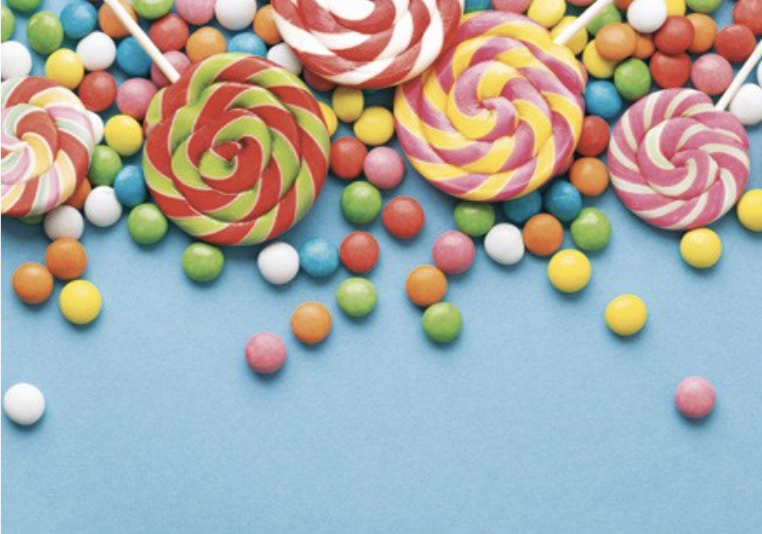
\includegraphics[width=0.9\textwidth]{bonbons.png}
\end{minipage}%

\vspace{10pt}

\noindent\hrulefill
\vspace{0.5cm}

\begin{center}
\textbf{Fin de l'interrogation — relire avant de rendre.}    
\end{center}

\end{document}
